\setcounter{chapter}{1}
\chapter*{Checklist instalace}

\ifthenelse{\equal{\kapitolaElektroinstalacniPrace}{1}}{	
    \section{Elektroinstalační práce}
    \begin{itemize}
        \item \textbf{Osazení a silové připojení EMS/DŘ rozvaděče} – jedná se o stavební montáž rozvaděče na určené místo definované 
        projektovou dokumentací. Dále pak připojení silových a signálních vodičů na svorky dle dokumentace.
         \ifthenelse{\equal{\rozvadecFullSVyhrivanim}{1}}{
        \item \textbf{Umístění rozvaděče EMS/DŘ} - pokud je rozvaděč umístěn ve venkovním prostředí, je vyžadováno aktivování vestavěného vyhřívání rozvaděče.}

        \item \textbf{Osazení a silové připojení MaR rozvaděče/čů} – jedná se o stavební montáž rozvaděče na určené místo definované projektovou dokumentací. Dále pak připojení silových a signálních vodičů na svorky dle dokumentace (řeší se pouze, pokud je obsažen v projektové dokumentaci). Rozvaděče zajišťují komunikaci, případně měření výrobních modulů a mají charakter podružného rozvaděče.
        \item \textbf{Počet skutečně instalovaných MaR rozvaděčů} – uveďte počet skutečně instalovaných rozvaděčů.
        \item \textbf{Osazení a silové připojení ELMĚR rozvaděče} – jedná se o stavební montáž rozvaděče na určené místo definované projektovou dokumentací. Dále pak připojení silových a signálních vodičů na svorky dle dokumentace (řeší se pouze, pokud je obsažen v projektové dokumentaci). Jedná se o podružný rozvaděč pro ty případy, kdy jsou MTP/MTN vzdálená v kabelové délce od EMS/DŘ rozvaděče dále než 20 m.
        \item \textbf{Označení rozvaděčů dle JPS} – uveďte názvy instalovaných rozvaděčů tak, jak jsou označeny na místě instalace. Tento název bude pak použit při konfiguraci.

    \end{itemize}
}


\ifthenelse{\equal{\kapitolaElektromery}{1}}{	
    \section{Elektroměry}
    \ifthenelse{\equal{\elektromerSMLvRozvadeci}{1}}{
        \subsection{Elektroměr SML133 v EMS/DŘ rozvaděči}
        \begin{itemize}
            \item \textbf{Osazení a připojení MTP} – jedná se o montáž měřicích transformátorů proudu (MTP). Trafa se montují na místa dle dokumentace o příslušném převodovém poměru. U montáže je nutné zkontrolovat správný převodový poměr, případně třídu přesnosti. 
            \item \textbf{Osazení a připojení MTN} – jedná se o montáž měřicích transformátorů napětí (MTN). Trafa se montují na místa dle dokumentace o příslušné velikosti. U montáže je nutné zkontrolovat správný převodový poměr, případně třídu přesnosti.
            \item \textbf{Kontrola správnosti směru toku proudu na MTP} – trafa je potřeba montovat v příslušném směru toku proudu, kdy správný směr je od distribuční sítě do odběrného místa, případně k výrobně.
            \item \textbf{Kontrola sledu fází} – je nutné dodržet správný sled fází L1-L2-L3
            \item \textbf{Kontrola příslušnosti napětí vs. proud} – je nutné dodržet vazbu mezi proudovými a napěťovými vstupy, tak aby měřený proud z fáze např. L1 odpovídal na napěťových svorkách elektroměru fázi L1 – viz schéma (pro příklad uveden elektroměr SML133)
            \vskip.2in
            \begin{minipage}{0.5\linewidth}
            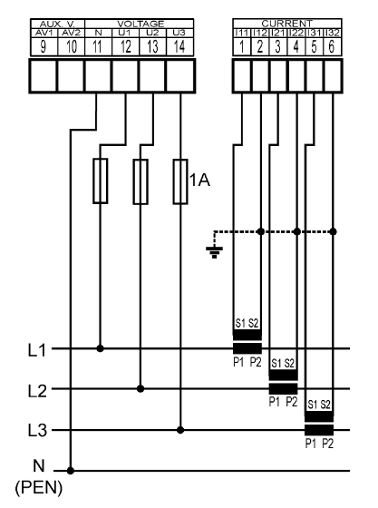
\includegraphics[width=0.9\linewidth]{img/navod/mtp.png}
            \captionof{figure}{Zapojení polopřímého měření (použítí MTP)}
            \end{minipage}
            \begin{minipage}{0.5\linewidth}
            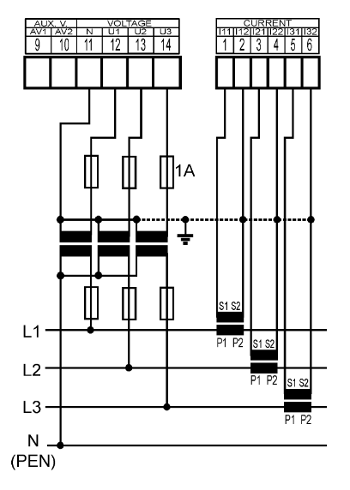
\includegraphics[width=0.9\linewidth]{img/navod/mtn.png}
            \captionof{figure}{Zapojení nepřímého měření (použití MTP a MTN)}
            \end{minipage}
            \item \textbf{Nastavení elektroměru} – elektroměr je potřeba nastavit dle místních parametrů a připojených MTP/MTN:
            \begin{itemize}
                \item Příklad nastavení MTP:

                \begin{minipage}{\linewidth}
                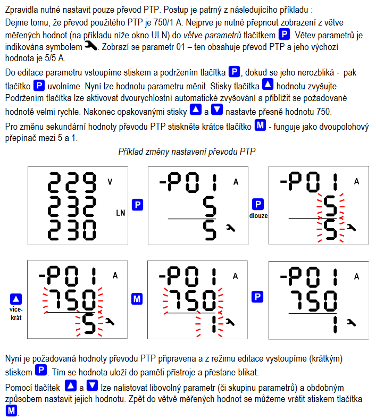
\includegraphics[width=\linewidth]{img/navod/nastavenimtp.png}
                %\captionof{figure}{Zapojení nepřímého měření (použití MTP a MTN)}
                \end{minipage}

                \item Přehled parametrů k nastavení: (01-05 je na displeji zastoupen P01-P05)

                \begin{minipage}{\linewidth}
                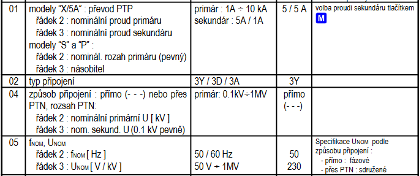
\includegraphics[width=\linewidth]{img/navod/nastavenip0105.png}
                %\captionof{figure}{Zapojení nepřímého měření (použití MTP a MTN)}
                \end{minipage}
            \end{itemize}

            \item Počet dalších instalovaných elektroměrů, např. pro měření FVE – uveďte počet dále instalovaných elektroměrů, např dílčí měření jednotlivých výrobních modulů.
            \item Informace k dalším instalovaných elektroměrům
            \begin{itemize}
                \item Označení elektroměru dle JPS – uveďte označení tak jak je uvedeno v JPS
                \item Typ elektroměru – uveďte přesný typ elektroměru (celý název)
                \item Způsob komunikace (Modbus RTU/TCP) – Modbus RTU využívá RS-485, Modbus TCP využívá datové sítě a elektroměr musí mít přidělenou IP adresu
                \item Připojeno k rozvaděči – v případě Modbus RTU uveďte, k jakému rozvaděči je elektroměr připojen
            \end{itemize}
        \end{itemize}

        \subsection{Podružné elektroměry}
        \begin{itemize}
            \item Nastavení dalších instalovaných elektroměrům
            \begin{itemize}
                \item Označení elektroměru dle JPS – uveďte označení tak jak je uvedeno v JPS
                \item Převodový poměr MTP (hodnota, je nastaveno v elektroměru) – uveďte hodnotu MTP a potvrďte nastavení hodnoty v elektroměru
                \item RTU adresa / IP TCP adresa  – uveďte příslušnou nastavenou adresu, buď ID adresu (RTU) nebo IP adresu (TCP)
                \item Ověřena korektnost zapojení – zde potvrzujete správné zapojení MTP (viz elektroměr SML133)
            \end{itemize}
        \end{itemize}

        

    }

}

\ifthenelse{\equal{\kapitolaParametrizaceKomunikace}{1}}{
    \section{Parametrizace a komunikace}
    \begin{itemize}
        \item Je nastavena datová síť pro komunikaci řídících jednotek – pro potřeby komunikace řídících jednotek s nadřazeným systémem je potřeba v rámci datové sítě nastavit příslušné parametry. Datová síť s přístupem na internet se připojuje na ETH 2 port řídící jednotky (případně na keystone RJ45/DIN). ETH 2 port řídicí jednotky je vyhrazen pro externí komunikaci, a to pro připojení k uživatelské aplikaci pomocí VPN, pro přístup k externím datovým zdrojům (synchronizace času, predikce solárního osvitu, počasí, ceny denního trhu apod.). Naše doporučení je připojit řídící jednotky do vyhrazené části sítě s možností komunikace do sítě internet. 
        \item Řídící jednotka má na ETH 2 portu zapnutý DHCP server pro přidělení IP adresy z nadřazeného serveru. Po připojení jednotky lze na displeji nalistovat položku ETH 2 a přečíst si přidělenou IP adresu. Doporučujeme daný IP rozsah rozdělit na část, která dynamicky přiděluje IP adresy od DHCP serveru a část, kde je vymezený rozsah pevně přidělený. Po připojení řídící jednotky do back-endu EnergoStation můžeme na jednotce vypnout DHCP a nastavit jí pevnou IP adresu dle požadavků místního IT. To doporučujeme udělat i pro ostatní technologii, s níž řídící jednotka komunikuje.
        \item \textbf{IP adresy a IC čísla řídících jednotek} – IC číslo je registrační číslo řídící jednotky v nadřazeném systému. Do tabulky je potřeba jej opsat a přiložit fotografii displeje při odeslání checklistu. K IC číslu se lze dostat po stisknutí tlačítka „Mode“, na displeji se objeví „RUN“. Následně šipkou dolů $\blacktriangledown$ (umístěna pod displejem) nalistovat displej viz obr.

        \begin{minipage}{\linewidth}
                \center
                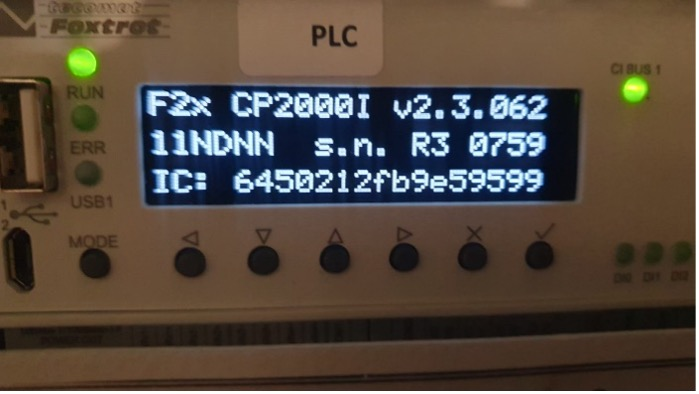
\includegraphics[width=0.5\linewidth]{img/navod/plc.jpg}
                %\captionof{figure}{Zapojení nepřímého měření (použití MTP a MTN)}
                \end{minipage}
        \end{itemize}
}

\ifthenelse{\equal{\kapitolaTechnologie}{1}}{
    \section{Technologie}

    \ifthenelse{\equal{\kapitolaTechnologieStridaceLogger}{1}}{
        \subsection{Střídače připojené přes Logger}
        \begin{itemize}
            \item \textbf{Připojení do datové sítě s viditelností na EMS/DŘ} - tyto typy zařízení komunikují pomocí Modbus TCP a je nutno jim nastavit správné parametry sítě a ověřit jejich viditelnost v síti.
            \item \textbf{Povoleno řízení loggeru nadřazeným systémem} - nadřazené loggery často vyžadují aktivaci povolení řízení tohoto zařízení nadřazeným systémem nebo 3tí stranou.
            \item \textbf{Připojení všdch řízených střídačů} – kontrola, zda v případě použití Smart loggeru nebo např. Data Hubu jsou k němu připojeny všechny střídače a komunikují s ním.
            \item Informace o střídačích a jejich adresace – zde vyplňte technické a datové parametry jednotlivých střídačů a loggerů.
            \begin{itemize}
                \item \textbf{Typ loggeru} – uveďte co nejpřesněji typové označení Data loggeru + přiložte foto štítku.
                \item \textbf{Sumární výkon střídačů} – jedná se o součet výkonů všech střídačů připojených do Data loggeru.
                \item \textbf{Výkon FVE} – jedná se o celkový výkon instalovaných panelů pod loggerem.
                \item \textbf{IP Adresa} - IP adresa v rámci sítě včetně portu na kterém běží na daném zařízení Modbus server.
                \item \textbf{Modbus ID} - ID zařízení v rámci Modbus sběrnice.
            \end{itemize}
        \end{itemize}
    }


    \ifthenelse{\equal{\kapitolaTechnologieStridaceRTU}{1}}{
        \subsection{Střídače připojené přes Modbus RTU}
        \begin{itemize}
            \item \textbf{Osazení zakončovacích odporů $120\ohm$ na koncích každé komunikační linky} – na sběrnici RS-485 je potřeba, aby poslední zařízení na konci větve mělo na svorkách RS-485 zakončovací odpor o velikosti 120 Ω. Na některých zařízeních lze zapnout tzv. vnitřní terminaci, která tuto funkci zajistí. Informace, zda Vámi instalované zařízení umí vnitřní terminaci, je nutné dohledat v dokumentaci výrobce. Pokud zařízení vnitřní terminaci nemá, je nutné instalovat zakončovací odpor na svorky RS-485 A/B.
            \item \textbf{Ověření polarity linek RS-485 (A, B, GND)} - v rámci instalace je nutné prověřit správnost polarity linky RS-485. Záleží na výrobci, jak má svorky RS-485 řazeny za sebou, ne vždy je řazení A, B, GND. Pokud nebude dodržena polarita, nebude komunikace fungovat.
            \item \textbf{Povoleno řízení střídačů přes Modbus} - střídače často vyžadují aktivaci povolení řízení tohoto zařízení nadřazeným systémem nebo 3tí stranou.
            \item \textbf{Připojení všdch řízených střídačů} – v případě použití Modbus RTU ověřit, zda jsou všechny střídače připojeny k příslušné sběrnici RS-485
        \end{itemize}
    }

    \ifthenelse{\equal{\kapitolaTechnologieStridaceTCP}{1}}{
        \subsection{Střídače připojené přes Modbus TCP}
        \begin{itemize}
            \item \textbf{Připojení do datové sítě s viditelností na EMS/DŘ} - tyto typy zařízení komunikují pomocí Modbus TCP a je nutno jim nastavit správné parametry sítě a ověřit jejich viditelnost v síti.
            \item \textbf{Povoleno řízení střídačů přes Modbus} - střídače často vyžadují aktivaci povolení řízení tohoto zařízení nadřazeným systémem nebo 3tí stranou.
            \item \textbf{Připojení všdch řízených střídačů} – pokud se jedná o připojení pomocí Modbus TCP, je potřeba mít na střídačích nastaveny příslušné parametry sítě a ověřit například pomocí příkazu „ping“ viditelnost na řídící jednotku.
        \end{itemize}
    }

    \ifthenelse{\equal{\kapitolaTechnologieBaterie}{1}}{
        \subsection{Bateriová úložiště}
        \begin{itemize}
            \item Jsou všechny prvky bateriového úložiště (střídače, BMS, atd.) připojeny k řídícím jednotkám – jedná se kontrolu zda všechny bateriové technologie jsou připojeny do stejné datové sítě jako řídící jednotky a je ověřena jejich viditelnost, např. pomocí příkazu ping na IP adresu hlavní řídící jednotky z místa připojení bateriové komponenty.
            \ifthenelse{\equal{\kapitolaTechnologieBaterieEMS}{1}}{
            \item Informace o bateriovém úložišti a adresace komponent
            \begin{itemize}
                \item \textbf{Typ / model bateriového úložiště} – uveďte typ bateriového uložiště co nejpřesněji + doplňte fotografií štítku. Pokud je BÚ složeno z více komponent rozepište se níže do tabulky a pořiďte foto z každé komponenty
                \item \textbf{Kapacita úložiště} – jedná se o celkovou kapacitu úložiště udávanou výrobcem
                \item \textbf{Max. SoC uložiště pro nabíjení} – jedná se o provozní maximální kapacitu, která většinou odpovídá 90-95% celkové kapacity. Nad tuto hranici se nesmí baterie nabít.
                \item \textbf{Min. SoC úložiště pro vybíjení} – jedná se o provozní minimální kapacitu, která většinou odpovídá 5-12% celkové kapacity. Pod tuto hranici se nesmí baterie vybít.
            \end{itemize}
            }

            \item Doplňující informace k bateriovému úložišti
            \begin{itemize}
                \item \textbf{Komponenta INV / BMS / MBMS} – jedná se o střídač, BMS, master BMS nebo jinou část bateriového úložiště. Přesné typové označení komponenty BÚ + doplněné o foto výrobního štítku
                \item \textbf{Kapacita BU} - jedná se o kapacitu bateriového úložiště dle štítku výrobce.
                \item \textbf{Max. výkon střídače} – jedná se o bateriový střídač a uveďte jeho maximální výkon.
                \item \textbf{Modbus ID} – pokud je střídač nebo jiná komponenta BÚ připojena na Modbus RTU, uveďte ID adresu. Pokud na Modbus TCP, uveďte IP adresu a ID.
                \item \textbf{ID úložiště} - bateriové úložiště může být připojené přímo, nebo začleněné do clusteru pod BMS - v takovém případě je identifikováno pomoci ID úložiště v rámci clusteru.            
            \end{itemize}
        \end{itemize}
    }
}


\ifthenelse{\equal{\kapitolaMeteostanice}{1}}{
    \section{Meteorologická stanice}
    \begin{itemize}
        \item \textbf{METEO stanice nainstalována s ohledem na měření osvitu elektrárny} – potvrzení, že METEO stanice byla instalována a připojena na datovou síť. Jedná se o montáž METEO stanice, která se instaluje na vyvýšené místo (např. střecha). METEO stanici je nutné připojit na datovou síť, přičemž datový kabel musí disponovat napájením, tzv. PoE.
        \item \textbf{IP adresa METEO stance je ve stejné síti jako EMS/DŘ} – u  stanice je nutno nastavit IP adresu dle parametrů LAN sítě ve které se nacházejí ostatní prvky (RTU, střídače, apod.). \newline Návod na nastavení IP adresy https://support.icool4.cz/a/solutions/articles/47001256155
        \item \textbf{IP adresa METEO stanice} – uveďte IP adresu, která byla nastavena do METEO stanice
    \end{itemize}
}


\ifthenelse{\equal{\kapitolaKompenzace}{1}}{
    \section{Kompenzace}
    \begin{itemize}
        \item Kompenzace a její ovládání bývá řešeno obvykle pouze tehdy, je-li to podmínka distributora nebo zákazníka.
    \end{itemize}
}


\setcounter{chapter}{2}
\setcounter{section}{0}
\chapter*{Nastavení systému}

Pro potřeby nastavení EMS/DŘ je potřeba vyplnit několik základních parametrů samotné služby „řízení energií“, obsluhovaných „zařízení“ (střídač, bateriové úložiště) a řízených „spotřebičů“ (proporcionálně řízená spirála akumulační nádrže, elektromobilita). Na základě uvedených hodnot bude nastaven a předán řídící systém EMS.

\ifthenelse{\equal{\kapitolaNastaveniOM}{1}}{
    \section{Parametry odběrného místa}
    \begin{itemize}
        \item \textbf{Jmenovitá hodnota hlavního jističe} – uveďte hodnotu hlavního jističe na předacím místě mezi odběrným místem a distribuční soustavou.
        \item \textbf{Hodnota rezervovaného příkonu dle SoP} – uveďte hodnotu rezervovaného příkonu z aktuální SoP.
        \item \textbf{Hodnota rezervovaného výkonu výrobny dle SoP} – uveďte hodnotu rezervovaného výkonu z aktuální SoP, jedná se o povolené přetoky do distribuční sítě.
        \item \textbf{Celkový instalovaný výkon dle SoP} – uveďte hodnotu celkového instalovaného výkonu z aktuální SoP.
        \item \textbf{Povolení přetoků do sítě během zkušebního provozu} – v případě, že na odběrném místě je již z minulosti instalovaný zdroj, je možné, že dle původní SoP jsou povoleny přetoky.
    \end{itemize}
}


\ifthenelse{\equal{\kapitolaNastaveniSPOT}{1}}{
    \section{Parametry SPOT / PRODEJ}

    \begin{itemize}
        \item Smlouva o dodávce elektřiny – prodej je – jaký obchodní vztah je na odběrném místě smluven. Řídí se odběrné místo SPOTem, nebo má fixní cenu elektřiny.
        \item \textbf{Zakázat dodávku do síte při záporných SPOT cenách} – v případě SPOTového smluvního vztahu má systém EMS blokovat dodávku do distribuční sítě při záporných cenách na SPOTu?
        \item Návod na výpočet: \newline https://support.energostation.com/a/solutions/articles/47001247456?lang=cs\&portalId=47000082337
    \end{itemize}

    \section{Parametry SPOT / NÁKUP}
    
    \begin{itemize}
        \item Smlouva o dodávce elektřiny – nákup je – jaký obchodní vztah je na odběrném místě smluven. Řídí se odběrné místo SPOTem, nebo má fixní cenu elektřiny.
        \item Návod na výpočet: \newline https://support.energostation.com/a/solutions/articles/47001247456?lang=cs\&portalId=47000082337
    \end{itemize}

    \vskip.2in
    \textbf{\textcolor{red}{!!! DŮLEŽITÉ:} pokud se bude nabíjet baterie ze SPOTu a OPM je fakturováno dle $1/4$h rezervované kapacity (RK), je nutné řešit sledování a řízení $1/4$h výkonu přímo z fakturačního elektroměru. Pokud nebude použito řízení $1/4$h rezervované kapacity z fakturačního elektroměru, je možné, že se limit RK překročí a OPM může být fakturováno za překročení limity RK.}
}


\ifthenelse{\equal{\kapitolaNastaveniRezerovaneKapacity}{1}}{
    \section{Parametry rezervované kapacity $1/4$h maxima}
    \begin{itemize}
        \item \textbf{Instalován a připojen galvanický optooddělovač pro sběr pulsů k fakturačnímu elektroměru} – jedná se o zařízení, které je instalováno co nejblíže fakturačního elektroměru. Jeho připojení k fakturačnímu elektroměru zajišťuje PDS. Instalace optooddělovače se řídí místními připojovacími podmínkami PDS.
        \item \textbf{Připojen galvanický optooddělovač k rozvaděči 1/4h maxima} – pro správnou funkčnost je nutné zajistit propojení mezi optooddělovačem a rozvaděčem ¼ hodinového maxima. Impulsy se připojují na vstupy prvku C-AM-0006I.
        \item \textbf{Připojen rozvaděč ¼ hod. maxima k EMS/DŘ rozvaděči} – jedná se komunikační připojení k EMS/DŘ rozvaděči pomocí CIB sběrnice, případně pomocí datové sítě.
        \begin{itemize}
            \item CIB adresa prvku AK.PULS (C-AM-0006I) – pokud se jedná o variantu s CIB propojením, je potřeba uvést CIB adresu prvku, kterou naleznete na samotném prvku.
            \begin{minipage}{\linewidth}
                \center
                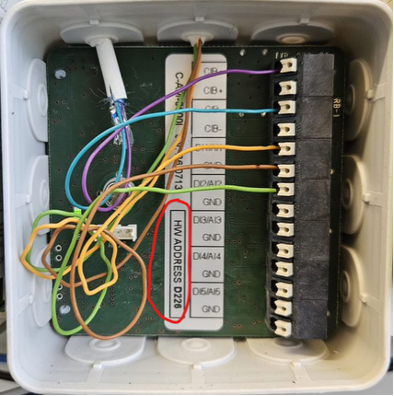
\includegraphics[width=0.5\linewidth]{img/navod/cam0006i.png}
                \captionof{figure}{TECO C-AM-0006I}
            \end{minipage}
        \end{itemize}
        
        \item \textbf{Popis pulsů} – uveďte jaký typ pulsu byl připojen kam. Musí odpovídat výstupu z FA elektroměru přes vstup do optooddělovače a následně jeho výstup. Většinou se připojuje synchronizační puls, A+, A-, případně jalový výkon
        \item \textbf{Regulativní stupně} – jedná se o definování technologií a pořadí v jakém se mají odpojovat či připojovat. Ovládání technologií může vyvolat dodatečné požadavky na HW a elektroinstalační práce.

    \end{itemize}
}



\ifthenelse{\equal{\kapitolaNastaveniBaterie}{1}}{
    \section{Nastavení bateriového úložiště}
   
}


\ifthenelse{\equal{\kapitolaNastaveniZdrojuEMS}{1}}{
    \section{Nastavení zdrojů EMS pro SPOT}
    
    \begin{itemize}
        \item \textbf{Povolit řízení EMS dle SPOT} – definujte, zda se májí technologie řídit SPOTem.
        \item \textbf{Povolit vybíjení baterie do sítě dle SPOT} – definujte, zda se má BÚ nabíjet a vybíjet dle SPOTu z/do sítě
        \item \textbf{Ztráty bateriového úložiště} – výrobcem definovaná procentuální vlastní ztráta BÚ
        \item \textbf{Jsou instalovány další zdroje do (EMS/DŘ)} – uveďte další zařízení, která nebyla zmíněna v rámci check-listu ve výše uvedených bodech
    \end{itemize}
}


